\subsection{实验目的-通过编写脚本配置防火墙}
通过编写脚本配置防火墙.
%
\subsection{实验原理}
编写脚本,执行脚本,完成防火墙的配置.
%
\subsection{实验环境}
操作系统: CentOS 6.5
%
\subsection{实验步骤}
\subsubsection{使用脚本配置防火墙}
在防火墙 CentOS 6.5 桌面新建 \texttt{firewall.sh},
在终端输入命令
\begin{minted}[bgcolor=bg,breaklines=true]{sh}
vi firewall.sh
\end{minted}
\begin{figure}[H]
  \begin{center}
    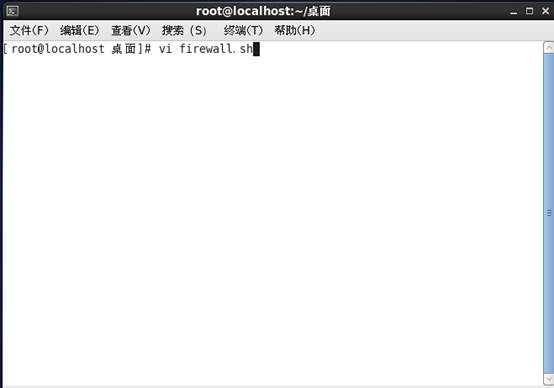
\includegraphics[width=0.40\textwidth]{2_8_1.jpeg}
  \end{center}
\end{figure}

编辑脚本 \texttt{firewall.sh},文件内容如下。
\begin{minted}[bgcolor=bg,breaklines=true]{sh}
#!/bin/bash
IPT="/sbin/iptables"
#Remove any existing rules
$IPT -F
$IPT -X
$IPT -Z
#setting for loopback interface
$IPT -t filter -A INPUT -i lo -j ACCEPT
$IPT -t filter -A OUTPUT -o lo -j ACCEPT
#setting default firewall policy
$IPT -P OUTPUT ACCEPT
$IPT -P FORWARD DROP
$IPT -P INPUT DROP
#setting access rules
$IPT -t filter -A INPUT -s 192.168.1.0/24 -p all -j ACCEPT
#http
$IPT -t filter -A INPUT -p tcp --dport 80 -j ACCEPT
#icmp
$IPT -t filter -A INPUT -p icmp -m icmp --icmp-type any -j ACCEPT
#others RELATED
$IPT -A INPUT -m state --state ESTABLISHED,RELATED -j ACCEPT
$IPT -A OUTPUT -m state --state ESTABLISHED,RELATED -j ACCEPT
\end{minted}
\begin{figure}[H]
  \begin{center}
    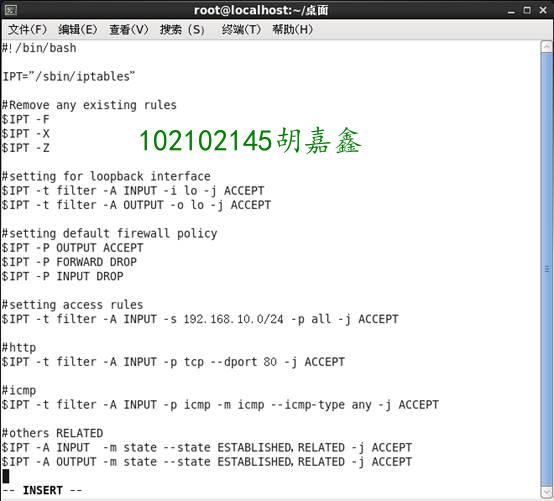
\includegraphics[width=0.40\textwidth]{2_8_2.jpeg}
  \end{center}
\end{figure}

此时在终端输入命令
\begin{minted}[bgcolor=bg,breaklines=true]{sh}
./firewall.sh
\end{minted}
执行脚本时提示权限不够,输入命令
\begin{minted}[bgcolor=bg,breaklines=true]{sh}
chmod +x firewall.sh
\end{minted}
为其添加权限。再执行脚本,则可执行成功。
\begin{figure}[H]
  \begin{center}
    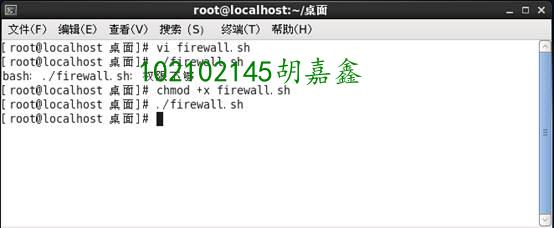
\includegraphics[width=0.40\textwidth]{2_8_3.jpeg}
  \end{center}
\end{figure}

在终端输入命令
\begin{minted}[bgcolor=bg,breaklines=true]{sh}
iptables -L -n --line-numbers
\end{minted}
查看防火墙规则,可以看到防火墙规则添加成功。
\begin{figure}[H]
  \begin{center}
    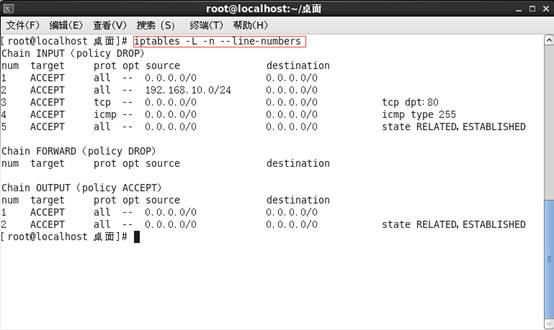
\includegraphics[width=0.40\textwidth]{2_8_4.jpeg}
  \end{center}
\end{figure}

但此时添加的防火墙规则只存在于内存中,
并没有写入 iptables 配置文件中。
一旦重启就会消失。将添加的防火墙规则永久保存在配置文件中,在终端输
入命令
\begin{minted}[bgcolor=bg,breaklines=true]{sh}
/etc/init.d/iptables save
\end{minted}
\begin{figure}[H]
  \begin{center}
    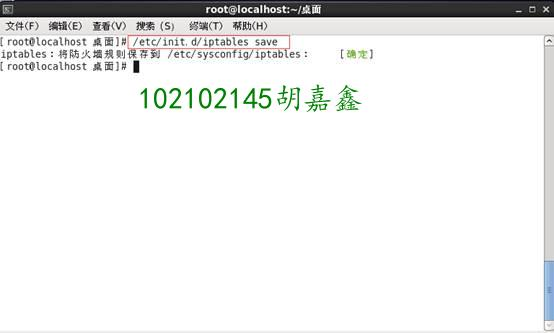
\includegraphics[width=0.40\textwidth]{2_8_5.jpeg}
  \end{center}
\end{figure}

在终端输入命令
\begin{minted}[bgcolor=bg,breaklines=true]{sh}
cat /etc/sysconfig/iptables
\end{minted}
查看 iptables 配置文件。
\begin{figure}[H]
  \begin{center}
    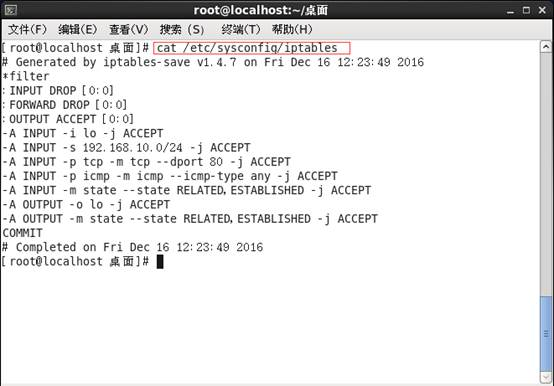
\includegraphics[width=0.40\textwidth]{2_8_6.jpeg}
  \end{center}
\end{figure}

可以看到此时的防火墙与手动执行 iptables
命令配置防火墙实验中配置防火墙一样。
相比于手动配置防火墙,使用脚本配置防火墙更加方便和快捷,
不用一条一条手动地添加规则。
